\documentclass{beamer}
%\usepackage[autokw=all]{svn-multi}
\setbeamertemplate{navigation symbols}{}
%\usetheme{Goettingen}
\usetheme{Malmoe}
\usefonttheme{default}
%\setbeamersize{text margin left=5pt,text margin right=5pt}

\usepackage{hyperref}
\usepackage{subfigure}
\usepackage{amsmath}
\usepackage{amssymb}
\usepackage{multimedia}
\usepackage{shadow}
%\usepackage{movie15}

\usepackage{tcolorbox}

% Create a ``Wider'' command to reduce margins.  Put
% ``\Wider{\lipsum[2]}'' in a frame...
\newcommand\Wider[2][3em]{%
\makebox[\linewidth][c]{%
  \begin{minipage}{\dimexpr\textwidth+#1\relax}
  \raggedright#2
  \end{minipage}%
  }%
}


%\usepackage[english]{babel}
%\usepackage{pgf,pgfarrows,pgfnodes,pgfautomata,pgfheaps}
% \usepackage[latin1]{inputenc}

\usepackage{graphicx}
\defbeamertemplate*{footline}{default theme}
{
  \leavevmode%
  \hbox{%
  \begin{beamercolorbox}[wd=.5\paperwidth,ht=2.25ex,dp=1ex,center]{author in head/foot}%
    %\usebeamerfont{author in head/foot}\insertshortauthor~~(\insertshortinstitute)
    \usebeamerfont{author in head/foot}\insertshortauthor
  \end{beamercolorbox}%
  \begin{beamercolorbox}[wd=.4\paperwidth,ht=2.25ex,dp=1ex,center]{title in head/foot}%
    \usebeamerfont{title in head/foot}\insertshorttitle
  \end{beamercolorbox}%
  \begin{beamercolorbox}[wd=.1\paperwidth,ht=2.25ex,dp=1ex,right]{date in head/foot}%
%    \usebeamerfont{page number}\insertframenumber{} / \inserttotalframenumber\hspace*{2ex} 
    \usebeamerfont{page number}\insertpagenumber{} / \insertpresentationendpage{} \hspace*{2ex} 
  \end{beamercolorbox}}%
  \vskip0pt%
}

\title[2-Photon Printing]{Progress report on 2-Photon Printing}

\author{Ben Pearre, Tim Otchy, Christos Michas}
%\institute[]{
%  Computer Science\\
%  University of Colorado at Boulder, USA}
\date{\today}
%\date{\today}

\begin{document}

\begin{frame}
  \titlepage
\end{frame}

\begin{frame}
  \frametitle{Outline}
  \tableofcontents
\end{frame}


%\begin{frame}
%  \outline
%\end{frame}

%%%%%%%%%%5%%%%%%%%%%5%%%%%%%%%%5
\section{Introduction}
\subsection{Goals}

\begin{frame}
  \frametitle{State of the art: NanoScribe}
  \begin{itemize}
  \item Resolution: $\left[ \begin{array}{ccc}0.5 & 0.5 & 1
    \end{array}\right]\mu m$
  \item Size: $300 \mu m^3$
    \begin{itemize}
    \item We can build larger structures
    \end{itemize}
  \item Speed:
    \begin{itemize}
    \item Full cube: 30 minutes
    \item Nerve cuff: 20 minutes
    \item Print speed depends on item's complexity
    \end{itemize}
  \item Structural limitations
  \item Proprietary
  \end{itemize}
\end{frame}


\begin{frame}
  \frametitle{Can we do better?  So far:}
  \begin{itemize}
  \item Resolution: variable! Currently e.g. $\left[ \begin{array}{ccc}\sim 6 & 0.2 & 1
    \end{array}\right]\mu m$ at $270 \mu m^3$
  \item Size: $\left[ \begin{array}{ccc} 270 & 270 & 450
    \end{array}\right]\mu m$
    \begin{itemize}
      \item Subject to how we hold the ipdip
    \item Can we build larger structures?
    \end{itemize}
  \item Speed:
    \begin{itemize}
    \item Full cube: 20 seconds
    \item Nerve cuff: 20 seconds
    \item Print speed depends on item's height, and $y$ and $z$ resolution
    \end{itemize}
  \item Structural limitations {\em might} be avoidable
  \item Open
  \end{itemize}
\end{frame}

%%%%%%%%%%5%%%%%%%%%%5%%%%%%%%%%
\section{Interface}

\begin{frame}
  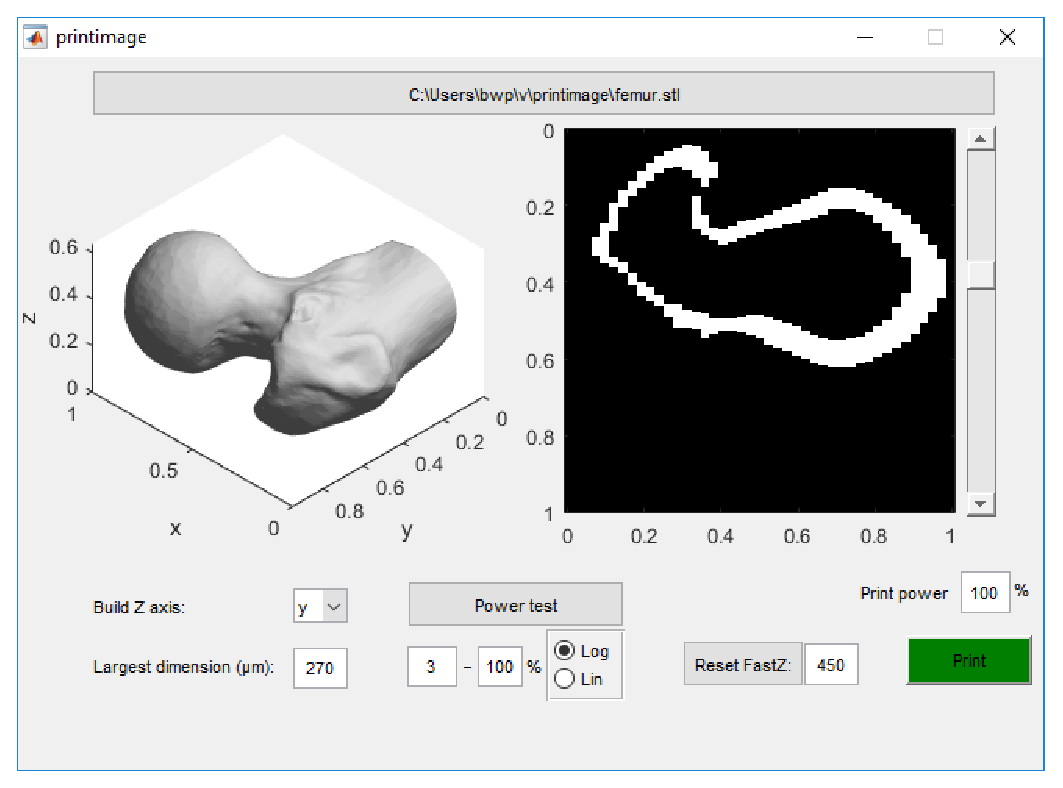
\includegraphics[width=\textwidth]{printimage}
\end{frame}

\begin{frame}
  \includegraphics[width=\textwidth]{powertest}
\end{frame}

\begin{frame}
  \includegraphics[width=\textwidth]{powertest-bubbles}
\end{frame}



%%%%%%%%%%5%%%%%%%%%%5%%%%%%%%%%
\section{Results}

\begin{frame}
  \includegraphics[height=\textheight]{cuffstuff}
\end{frame}

\begin{frame}
  \includegraphics[width=\textwidth]{printed-femur}
\end{frame}

\begin{frame}
  \includegraphics[width=\textwidth]{femur-closeup}
\end{frame}

\begin{frame}
  \includegraphics[width=\textwidth]{einsteins-etc}
\end{frame}

\begin{frame}
  \includegraphics[width=\textwidth]{cuff}
\end{frame}

\begin{frame}
  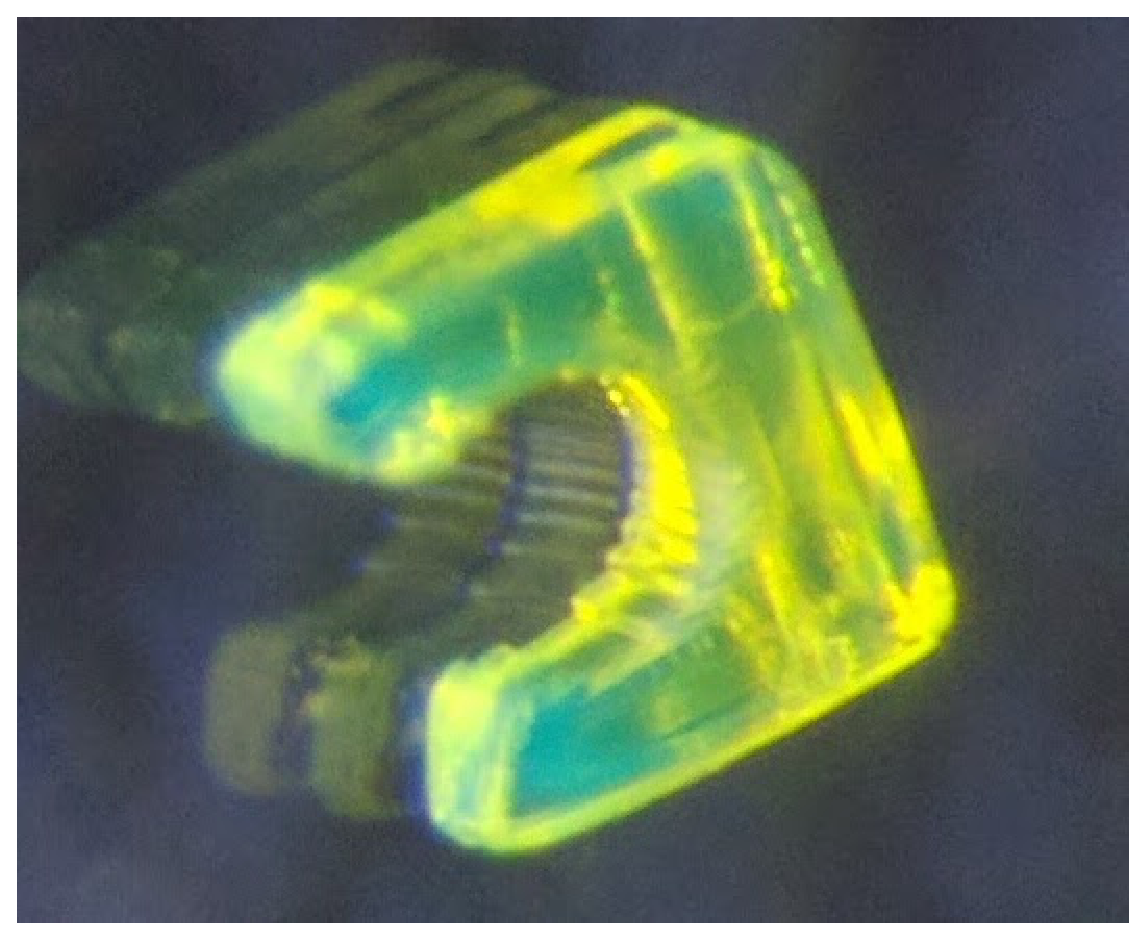
\includegraphics[width=\textwidth]{cuff-optical}
\end{frame}



%%%%%%%%%%5%%%%%%%%%%5%%%%%%%%%%
\section{Future work}

\begin{frame}
  \frametitle{To be continued\dots}
  \begin{itemize}
  \item Maybe don't crush printed objects?
  \item Power can compensate for resonant scanner's dwell time variability
  \item Superimpose to-be-printed on top of current image
  \item More reliable $z$ alignment
  \item Better viewing
    \begin{itemize}
    \item Power
    \item Wavelength
    \item Working distance
    \end{itemize}
  \item Higher $x$ resolution
  \item Higher $z$ resolution?
  \item Use motor stage to print larger parts
  \end{itemize}
\end{frame}
  
\end{document}
